
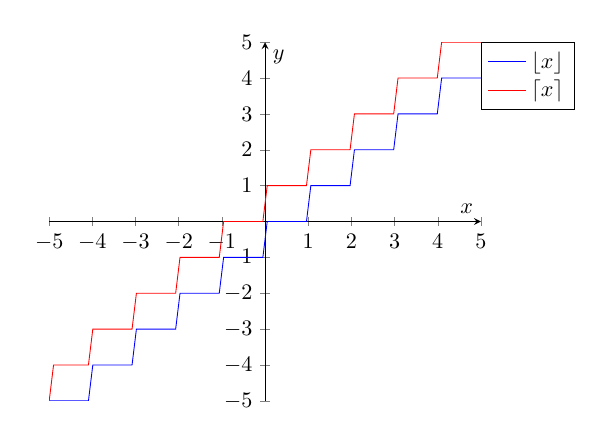
\begin{tikzpicture}[scale=0.8]
    \begin{axis}[
      xlabel=$x$,
      ylabel=$y$,
      axis lines=middle,
      ymin=-5, ymax=5,
      xmin=-5, xmax=5,
      xtick={-5,-4,-3,-2,-1,0,1,2,3,4,5},
      ytick={-5,-4,-3,-2,-1,0,1,2,3,4,5},
      legend pos=north west,
      legend style={at={(1,1)},anchor=north west}
    ]
    
    % Floor function
    \addplot[color=blue,domain=-5:5,samples=100] {floor(x)};
    \addlegendentry{$\lfloor x \rfloor$}
    
    % Ceiling function
    \addplot[color=red,domain=-5:5,samples=100] {ceil(x)};
    \addlegendentry{$\lceil x \rceil$}
    
    \end{axis}
  \end{tikzpicture}